\subsection{Parameter Evolution} \label{Sec: Parameter Evolution}
In this section, we discuss the parameter evolution of the Saunders luminosity function fits in Figure \ref{Fig: Bolometric IR LF}. The evolution of $\phi^{*}$ and $L^{*}$ across redshift is presented in Figure \ref{Fig: Param Evo} with values and errors in Table \ref{Tab: Param Evo}. The best fitting parameter values were calculated following the same fitting routine outlined in Section \ref{Sec: Bolometric IR LF}. As discussed in section \ref{Sec: Bolometric IR LF}, our final redshift bin likely suffers from incompleteness. However, ZFOURGE's ability to probe fainter luminosities becomes advantageous at higher redshifts, providing more reliable constraints on the LF parameters.

To better constrain the faint end slope of all LFs presented in this work, we fix $\alpha=1.3$ across all redshift bins. This result differs from the literature where \cite{rodighiero_mid-_2010, gruppioni_herschel_2013} fix $\alpha=1.2$ whereas \cite{fu_decomposing_2010} leaves $\alpha$ as a free fitting parameter found to be $\alpha=1.46$ (respective to our Saunders fitting function). This is because our LFs extend much further at the faint end. However, as we lack luminosity bins along the bright end of the LF, we fix the bright end $\sigma$ to values that fit best to the available literature. The faint end slopes of CIGALE LFs agree with the literature. Due to the absence of bright-end AGN luminosity bins, we incorporate data from \cite{thorne_deep_2022} to help constrain the AGN LF fitting process.

\begin{figure}[h]
    \centering
    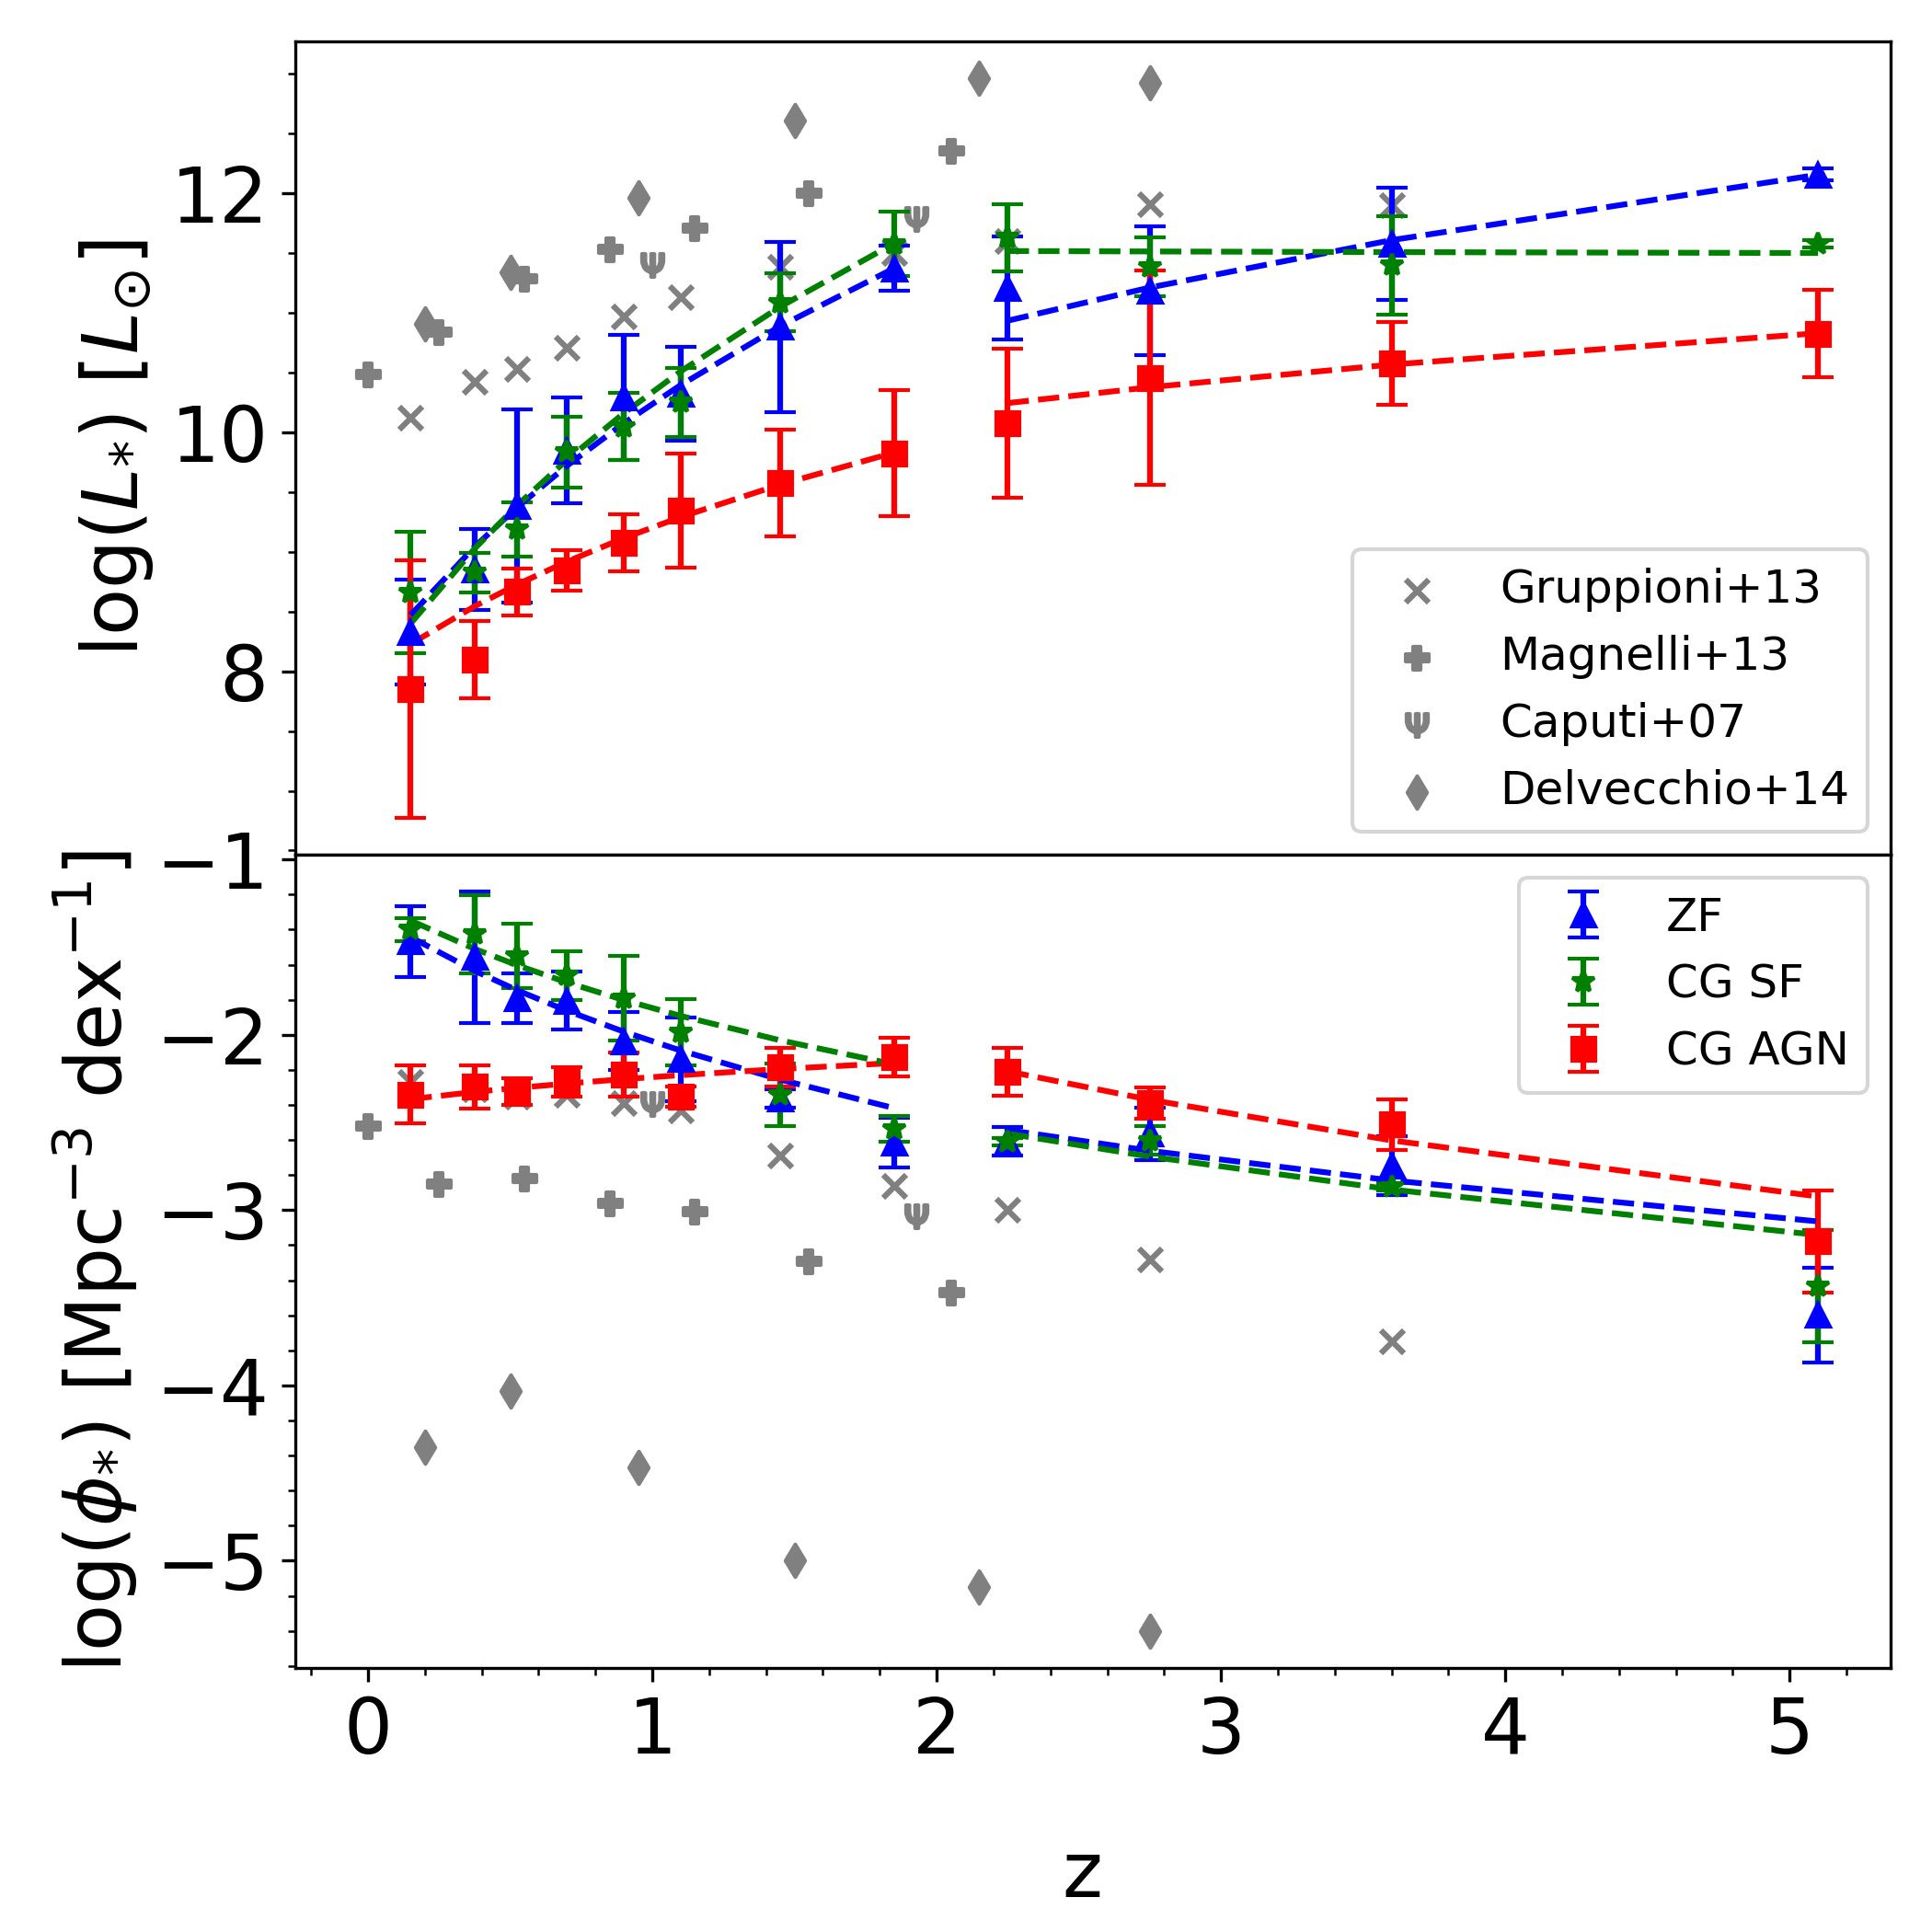
\includegraphics[width=0.48\textwidth]{Figures/Param_Evo.png}
    \caption{Best fitting parameters and uncertainties to our luminosity functions. Top: $L^{*}$ evolution. Bottom: $\phi^{*}$ evolution. Blue triangles represent the ZFOURGE. Red squares represent the CIGALE AGN and green stars the CIGALE SF population. Dashed lines represent the $\propto(1+z)^k$ evolution. We compare our results to the relevant literature, which is coloured grey. \cite{gruppioni_herschel_2013} crosses, \cite{magnelli_deepest_2013} pluses, and \cite{caputi_infrared_2007} uppercase $\Psi$'s.}
    \label{Fig: Param Evo}
\end{figure}

\begin{table}[h]
    \caption{Best-fit and fixed Saunders parameters for each LF across different redshift bins.}
    \label{Tab: Param Evo}
    \begin{center}
    \begin{tabular}{ccccc}
        \toprule
        $z$ & log$(L^{*})$ & log$(\phi^{*})$ & $\alpha$ & $\sigma$ \\
        \hline
        ZFOURGE \\
        \hline
        0.00 $\leq z <$ 0.30 &  8.33 $\pm$ 0.44 & -1.47 $\pm$ 0.20 & 1.3 & 1.1 \\
        0.30 $\leq z <$ 0.45 &  8.85 $\pm$ 0.34 & -1.56 $\pm$ 0.37 & 1.3 & 1.0 \\
        0.45 $\leq z <$ 0.60 &  9.38 $\pm$ 0.81 & -1.79 $\pm$ 0.14 & 1.3 & 0.9 \\
        0.60 $\leq z <$ 0.80 &  9.84 $\pm$ 0.44 & -1.81 $\pm$ 0.17 & 1.3 & 0.8 \\
        0.80 $\leq z <$ 1.00 & 10.29 $\pm$ 0.52 & -2.04 $\pm$ 0.17 & 1.3 & 0.7 \\
        1.00 $\leq z <$ 1.20 & 10.32 $\pm$ 0.39 & -2.14 $\pm$ 0.24 & 1.3 & 0.7 \\
        1.20 $\leq z <$ 1.70 & 10.88 $\pm$ 0.71 & -2.36 $\pm$ 0.05 & 1.3 & 0.7 \\
        1.70 $\leq z <$ 2.00 & 11.37 $\pm$ 0.19 & -2.61 $\pm$ 0.14 & 1.3 & 0.7 \\
        2.00 $\leq z <$ 2.50 & 11.21 $\pm$ 0.43 & -2.61 $\pm$ 0.08 & 1.3 & 0.7 \\
        2.50 $\leq z <$ 3.00 & 11.18 $\pm$ 0.54 & -2.56 $\pm$ 0.15 & 1.3 & 0.7 \\
        3.00 $\leq z <$ 4.20 & 11.57 $\pm$ 0.47 & -2.75 $\pm$ 0.17 & 1.3 & 0.7 \\
        4.20 $\leq z <$ 6.00 & 12.16 $\pm$ 0.05 & -3.60 $\pm$ 0.27 & 1.3 & 0.7 \\     
        \hline 
        CIGALE AGN \\
        \hline 
        0.00 $\leq z <$ 0.30 &  7.85 $\pm$ 1.08 & -2.34 $\pm$ 0.16 & 1.3 & 1.4 \\
        0.30 $\leq z <$ 0.45 &  8.10 $\pm$ 0.33 & -2.30 $\pm$ 0.12 & 1.3 & 1.3 \\
        0.45 $\leq z <$ 0.60 &  8.66 $\pm$ 0.20 & -2.32 $\pm$ 0.08 & 1.3 & 1.2 \\
        0.60 $\leq z <$ 0.80 &  8.84 $\pm$ 0.17 & -2.27 $\pm$ 0.08 & 1.3 & 1.1 \\
        0.80 $\leq z <$ 1.00 &  9.07 $\pm$ 0.24 & -2.23 $\pm$ 0.13 & 1.3 & 1.0 \\
        1.00 $\leq z <$ 1.20 &  9.34 $\pm$ 0.48 & -2.35 $\pm$ 0.06 & 1.3 & 0.9 \\
        1.20 $\leq z <$ 1.70 &  9.57 $\pm$ 0.44 & -2.18 $\pm$ 0.11 & 1.3 & 0.9 \\
        1.70 $\leq z <$ 2.00 &  9.82 $\pm$ 0.53 & -2.13 $\pm$ 0.11 & 1.3 & 0.9 \\
        2.00 $\leq z <$ 2.50 & 10.07 $\pm$ 0.62 & -2.21 $\pm$ 0.14 & 1.3 & 0.8 \\
        2.50 $\leq z <$ 3.00 & 10.46 $\pm$ 0.89 & -2.39 $\pm$ 0.09 & 1.3 & 0.7 \\
        3.00 $\leq z <$ 4.20 & 10.57 $\pm$ 0.35 & -2.51 $\pm$ 0.15 & 1.3 & 0.7 \\
        4.20 $\leq z <$ 6.00 & 10.82 $\pm$ 0.37 & -3.18 $\pm$ 0.29 & 1.3 & 0.7 \\
        \hline
        CIGALE SF \\
        \hline
        0.00 $\leq z <$ 0.30 &  8.66 $\pm$ 0.51 & -1.40 $\pm$ 0.07 & 1.3 & 1.1 \\
        0.30 $\leq z <$ 0.45 &  8.83 $\pm$ 0.17 & -1.43 $\pm$ 0.22 & 1.3 & 1.0 \\
        0.45 $\leq z <$ 0.60 &  9.19 $\pm$ 0.23 & -1.55 $\pm$ 0.18 & 1.3 & 0.9 \\
        0.60 $\leq z <$ 0.80 &  9.83 $\pm$ 0.30 & -1.66 $\pm$ 0.14 & 1.3 & 0.8 \\
        0.80 $\leq z <$ 1.00 & 10.05 $\pm$ 0.28 & -1.79 $\pm$ 0.24 & 1.3 & 0.7 \\
        1.00 $\leq z <$ 1.20 & 10.25 $\pm$ 0.29 & -1.99 $\pm$ 0.19 & 1.3 & 0.7 \\
        1.20 $\leq z <$ 1.70 & 11.08 $\pm$ 0.24 & -2.34 $\pm$ 0.18 & 1.3 & 0.7 \\
        1.70 $\leq z <$ 2.00 & 11.58 $\pm$ 0.27 & -2.53 $\pm$ 0.07 & 1.3 & 0.7 \\
        2.00 $\leq z <$ 2.50 & 11.63 $\pm$ 0.28 & -2.61 $\pm$ 0.02 & 1.3 & 0.7 \\
        2.50 $\leq z <$ 3.00 & 11.54 $\pm$ 0.25 & -2.70 $\pm$ 0.08 & 1.3 & 0.7 \\
        3.00 $\leq z <$ 4.20 & 11.40 $\pm$ 0.41 & -2.87 $\pm$ 0.02 & 1.3 & 0.7 \\
        4.20 $\leq z <$ 6.00 & 11.57 $\pm$ 0.03 & -3.43 $\pm$ 0.32 & 1.3 & 0.7      
        \botrule
    \end{tabular}
    \end{center}
\end{table}

Our ZFOURGE free parameters $L^{*}$ and $\phi^{*}$ exhibit evolutionary trends that differ from those reported in the literature. However, our fitting process is robust, and the evolution of the free parameters does not change significantly when the fixed parameters are altered. A known challenge in this analysis is the degeneracy between $L^{*}$ and $\phi^{*}$. A decrease in $L^{*}$ can be somewhat compensated for by increasing $\phi^{*}$ and vice-versa. Thus, the absolute values of the parameters themselves can be overlooked in favour of the overall trend in the dataset. 

As shown below, we find rapid evolution of ZFOURGE $L^{*}$ up to $z\approx2$, after which $L^{*}$ evolution slows. ZFOURGE $\phi^{*}$ shows consistent evolution in all redshift bins: 

\begin{equation*}
    L^{*}_{ZF} =
    \begin{cases} 
        10^{8.02 \pm 0.11} \times (1+z)^{7.36 \pm 0.25} & \text{for } z < 2, \\
        10^{8.65 \pm 0.31} \times (1+z)^{4.47 \pm 0.40} & \text{for } z > 2.
    \end{cases}
\end{equation*}

\begin{equation*}
    \phi^{*}_{ZF} =
    \begin{cases} 
        10^{-1.29 \pm 0.04} \times (1+z)^{-2.47 \pm 0.26} & \text{for } z < 2, \\
        10^{-1.57 \pm 0.59} \times (1+z)^{-1.91 \pm 1.04} & \text{for } z > 2.
    \end{cases}
\end{equation*}

Compared to the literature, both \cite{gruppioni_herschel_2013} and \cite{magnelli_deepest_2013} find much shallower $L^{*}$ evolution from $0<z<1$. ZFOURGE evolves 2-3x faster at $0<z<1$, but only 1.25x faster at $z>1$. This could be explained by ZFOURGE probing fainter luminosities. However, it is important to note that ZFOURGE was optimised for studying galaxies at $z>1$, where its deep near-infrared coverage is particularly effective. Consequently, results at $z<1$ should be interpreted cautiously, as the survey's design is less tailored to these lower redshifts. 

The CIGALE SF $L^{*}$ presents similar evolution compared to the ZFOURGE from $0<z<2$. In contrast to ZFOURGE results, the CIGALE SF $L^{*}$ declines from $z>2$ onwards. 

\begin{equation*}
    L^{*}_{SF} =
    \begin{cases} 
        10^{7.91 \pm 0.16} \times (1+z)^{8.07 \pm 0.37} & \text{for } z < 2, \\
        10^{11.55 \pm 0.47} \times (1+z)^{-0.06 \pm 0.73} & \text{for } z > 2.
    \end{cases}
\end{equation*}

This reversal is not seen in the evolution of $\phi^{*}$, which has a similar slope across all redshifts and is almost identical to ZFOURGE. 

\begin{equation*}
    \phi^{*}_{SF} =
    \begin{cases} 
        10^{-1.22 \pm 0.05} \times (1+z)^{-2.08 \pm 0.33} & \text{for } z < 2, \\
        10^{-1.48 \pm 0.46} \times (1+z)^{-2.21 \pm 0.81} & \text{for } z > 2.
    \end{cases}
\end{equation*}

The reversal in the evolution of $L^{*}$ below $z>2$ indicates that SF grew from at least $z=5$ to $z=2$ and has been declining ever since. It is well known (\citealp{gruppioni_herschel_2013,  madau_cosmic_2014} and references within) that the IR luminosity density has been declining since $z\approx2$ and we explore this more in Section \ref{Sec: IR Density}. 

% \cite{gruppioni_herschel_2013} and \cite{magnelli_deepest_2013} find similar results in $L^{*}$ from $0<z<1$ and similar $\phi^{*}$ evolution from $0<z<2$. 

We consistently see that, according to the evolution of $\phi^{*}$, the number of SF galaxies has increased since cosmic dawn. However, the characteristic luminosity $L^{*}$, has been declining since $z\approx2$. This shows that fainter SF galaxies become more common in the local universe. Our results reaffirm that $z\approx2$ is an important epoch for galaxy evolution.

The CIGALE AGN $L^{*}$ and $\phi^{*}$ evolve differently from the literature and from our ZFOURGE and CIGALE SF parameters at $z<2$:

\begin{equation*}
    L^{*}_{AGN} =
    \begin{cases} 
        10^{7.98 \pm 0.07} \times (1+z)^{4.06 \pm 0.17} & \text{for } z < 2, \\
        10^{9.15 \pm 0.24} \times (1+z)^{2.14 \pm 0.33} & \text{for } z > 2.
    \end{cases}
\end{equation*}

\begin{equation*}
    \phi^{*}_{AGN} =
    \begin{cases} 
        10^{-2.4 \pm 0.05} \times (1+z)^{0.52 \pm 0.16} & \text{for } z < 2, \\
        10^{-0.87 \pm 0.29} \times (1+z)^{-2.61 \pm 0.52} & \text{for } z > 2.
    \end{cases}
\end{equation*}

At $z>2$, the evolution of $L^{*}$ follows a similar trend to ZFOURGE, and a slower evolution at $z<2$. $\phi^{*}$ evolves similarly to SF and ZFOURGE at $z>2$. However, we see a reversal in the evolution of $\phi^{*}$ at $z<2$. This anomalous behaviour could be attributed to the degeneracy between $L^{*}$ and $\phi^{*}$. However, the magnitude of this degeneration has not been observed so prominently in the literature, suggesting two possibilities: CIGALE reveals a significant evolutionary epoch for AGN at $z<2$, or there is a bias in our fitting process. Our fitting process produces similar results for the ZFOURGE as seen in the literature and recovers the peak and turnover in the CIGALE SF, proving that $z<2$ is a significant epoch for AGN evolution. \cite{hopkins_observational_2007} and \cite{delvecchio_tracing_2014} show a similar reversal and subsequent decline in $\phi^{*}$ evolution below $z=1$. \cite{katsianis_evolution_2017} shows that high SFG rapidly decline below $z\approx1$ because of AGN feedback. We are therefore confident in our CIGALE AGN results. Our results imply fewer AGN in the local universe and are significantly fainter than in the early universe. 

Our results are complex, but showcase the importance of decomposing the SED of galaxies to separate the SF and AGN components. These trends indicate significant shifts in AGN and SF activity over cosmic time that were not detected in the combined ZFOURGE evolution.

% Our ZFOURGE findings indicate that the universe evolved slowly above redshift $z \approx 1$ when the universe was $\approx6$ Gyrs old. Since then, the characteristic luminosity, $L_{*}$, decreased substantially from $2.96\times10^10 L_{\odot}$ at $z=1.1$ to $2.19\times10^8 L_{\odot}$ at $z=0.15$ when the universe was $\approx11.5$ Gyrs old. This represents a 134x decrease in the characteristic luminosity across this time period. in the number density of galaxies between these two times. The characteristic luminosity, $L_{*}$, similarly shows little evolution above $z=2$ and evolves rapidly at lower redshifts. 

% \begin{itemize}
%     \item \textcolor{red}{Did we use literature data to constrain fits?}
%     \item \textcolor{red}{parameter degeneracy}
%     \item \textcolor{red}{evolution as $(1+z)^{k}$}
% \end{itemize}

% The degeneracy between $L^{*}$ and $\phi^{*}$ exists, but the shape of their evolution is largely consistent across the literature \citep{gruppioni_herschel_2013, magnelli_deepest_2013}.

% From $0<z<1$, ZFOURGE characteristic luminosity $L^{*}$ increases by 134x. From $1<z<5$, another 118x increase is seen. ZFOURGE $\phi^{*}$ decreases by 4x and 47x over the same time period. These redshift ranges represent $\approx5$ Gyrs and $\approx4$ Gyrs of evolution respectively. Thus, ZFOURGE $L^{*}$ evolution remains roughly constant over the universe's lifetime. ZFOURGE characteristic density $\phi^{*}$ shows significant evolution.

% CIGALE SF $L^{*}$ increases by 8x from $0<z<1$ and another 8x from $1<z<2$. From $2<z<5$ $L^{*}$ decreases by 4x. $\phi^{*}$ decreases by 2x, another 2x, and 3.5x over the same period. These redshifts represent 5, 2, and 2 Gyrs of evolution respectively. 

% CIGALE AGN $L^{*}$ initially decreases by 1.3x from $0<z<1$ and increases by 66x from $1<z<5$. AGN $\phi^{*}$ increases by 2.4x from $0<z<1$ and decreases by 11.4x from $1<z<5$.